\documentclass[a4paper]{article}
\usepackage[utf8]{ctex}
\usepackage{amsmath}
\usepackage{amsfonts}
\usepackage{graphicx}

\title{\textbf{作业八:Bellman-Ford算法的实现}}
\author{李沁霞 \\ 3210300363 统计学}
\date{\today}

\begin{document}

\maketitle

\section{简介}
Bellman-Ford算法的实现与其他动态规划问题一样,该算法以自下而上的方式计算最短路径。它首先计算路径中最多有一条边的最短距离。然后,他计算多有2条边的最短路径,以此类推。在外循环的第i次迭代之后,计算最多i条边的最短路径。可以有最大值|V|任何简单路径中的1个边,这就是外循环运行|v|的原因-1次。\\
\\
下面是算法的步骤:
\begin{enumerate}
    \item 让给定的源顶点为0。除了源点距离,将所有距离初始化为无限。
    \item 让所有边按照顺序处理。当第一次处理所有边时,我们得到初始距离。再次处理所有边,当不能改变所有边的距离才完成迭代。
\end{enumerate}

\section{测试结果}
\begin{tabular}{|c|c|c|c|c|}
    \hline
     V &  500 & 1000 & 2000 & 4000 \\
     \hline
     E = 2*|V| & 0.014 & 0.05 & 0.268 & 1.049 \\
     E = 4*|V| & 0.019 & 0.101 & 0.386 & 1.871 \\
     E = 8*|V| & 0.024 & 0.15 & 0.636 & 4.646 \\
     E = 16*|V| & 0.07 & 0.341 & 2.039 & 21.845 \\
     \hline
\end{tabular}
\begin{center}
    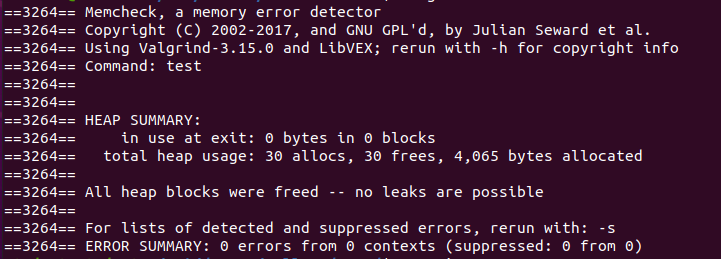
\includegraphics[scale= 0.5]{leaks}
\end{center}

\end{document}
